\documentclass{jeb}
\usepackage{graphics}
\usepackage{placeins}

\newcommand{\Hyalepugettensis}{\Genus{Hyale pugettensis}}
\newcommand{\Hpugettensis}{\Genus{H.~pugettensis}}
\newcommand{\Hyale}{\Genus{H.~pugettensis}}
\newcommand{\Parhyalehawaiensis}{\Genus{Parhyale hawaiensis}}
\newcommand{\Phawaiensis}{\Genus{P.~hawaiensis}}
\newcommand{\Parhyale}{\Genus{P.~hawaiensis}}
\newcommand{\degree}{$^\circ$}

\jebtitle{The jump of the amphipod \Hyalepugettensis:  Kinematics and the mechanism of jumping}

\jebauthorlist{
\jebauthor{Dennis~Evangelista}{1,*},
\jebauthor{Michael W. Perry}{1} and
\jebauthor{Charline Ng}{1}}

\jebaffiliationlist{
\jebaffiliation{1}{Department of Integrative Biology, University of California, Berkeley, 3060 Valley Life Sciences Building \#3140, Berkeley, CA 94720-3140, USA}}

\jebcontact{email: devangel@berkeley.edu}

\jebsummary{Kinematics of jumping amphipods (\Hyalepugettensis) were obtained with high speed video and analyzed for jump distance, energetics, and power requirements.  \Hyale\ were found to be passive spinning projectiles once in the air, taking off at a muzzle velocity of \unitfrac[100]{body lengths}{s} and spinning at \unit[2000]{rpm}.  Takeoff accelerations reached \unitfrac[221]{m}{s$^{\textsf{2}}$}, approximately 23 G's.  Takeoff was accomplished with a rapid abdominal extension, and required such high specific power output (\unitfrac[1100]{W}{kg}) that an elastic storage mechanism must be present.  Anatomical studies suggest several possible storage mechanisms and triggers to examine in future work.  A mathematical model of the initial instant of launch, also applicable to other jumping organisms that use abdominal extension, is described.  {\em Other observed tail behaviors are also reported?  Other species and transition to terrestriality in Talitridae?}}

\jebkeywords{\Hyalepugettensis, amphipod, jumping, biomechanics,}

\jebshorttitle{Amphipod jumping}
\jebshortnames{D. Evangelista and others}





\begin{document}
\maketitle

\section{Introduction}
Jumping has been studied in a wide range of small terrestrial arthropods, including fleas \citep{Bennet-Clark:1967},  locusts \citep{Bennet-Clark:1975}, various hemiptera \citep{Burrows:2006a, Burrows:2006, Burrows:2007, Burrows:2008, Burrows:2008a}, springtails \citep{Christian:1978}, millipedes \citep{Evans:1973}, bristletails \citep{Evans:1975}, click beetles \citep{Evans:1972, Makings:1973}, cicadas \citep{Gorb:2004} and trap jaw ants \citep{Gronenberg:1996, Patek:2006}.  Small jumpers often have such high specific power output that they require elastic storage mechanisms and triggers \citep{Bennet-Clark:1975a, Gronenberg:1996}.  Studies of jumping biomechanics in amphipods would be an interesting addition because they are a lineage that has come ashore, with living members who are fully marine, freshwater, semi-terrestrial, and fully terrestrial \citep{Hurley:1968, Spicer:1987}.  

Of the amphipods, talitrid amphipods such as beach hoppers (\Genus{Orchestia cavimana}), \Genus{Talitrus}, or \Genus{Hyale}, have been the subject of studies regarding ecology, phylogeny, physiology and behavior, but only \citet{Bracht:1980} examined the biomechanics of jumping directly.  \citet{Bracht:1980} filmed \Genus{Orchestia}\ at 1000 frames s$^-1$ and found jumping was accomplished by rapid abdominal extension.  This mode of jumping is convergent with that used in bristletails \citep{Evans:1975} and springtails \citep{Christian:1978}, both basal wingless hexapods.  In \Genus{Orchestia}, jumps lasted 350 to 400 ms and had an average distance of 18 cm and average launch velocity of 1.48 m/s \citep{Bracht:1980}.  While pioneering as a study of jumping amphipod biomechanics, conclusions about a two-phase extension of the abdomen were based on questionable differentiation of kinematic data \citep{Crenshaw:2000}.  \citet{Bracht:1980} also stated, without providing evidence, that \Genus{Orchestia} was unable to control itself in the air.  
	
Taking previous studies of \Genus{Orchestia}~as a starting point, we examined jumping in \Hyalepugettensis, a basal talitrid amphipod local to Friday Harbor, San Juan Island, WA.  This paper describes use of kinematics from high speed video and mathematical modeling to test the hypotheses that (1) As in many other wingless arthropods, aerial control exists in amphipods; (2) Abdominal extensor muscles power jumping \citep{Bracht:1980}; and (3) Jumping is related to escape swimming or other tail movements??? 

\section{Materials and methods}
\subsection{Animals}
	Specimens of the talitrid amphipod \Hyalepugettensis~(Fig.~\ref{fig:1}) were collected from tide pools in two locations, Friday Harbor Labs and Cattle Point, both on San Juan Island, WA (Fig.~\ref{fig:2}).  Amphipods were maintained in flow-through seawater tables at 12\degC with a natural daylight cycle and fed \Genus{Ulva}~and \Genus{Polysiphonia}~\emph{ad libitum}.  A summary of the mass, length, and height of animals collected is given in Table~\ref{table:1}.
\begin{figure}
\begin{center}
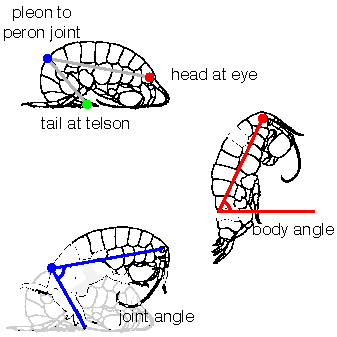
\includegraphics{figures/HyaleLandmarks.pdf}
\end{center}
\caption{Hyale drawing and landmarks etc.}
\end{figure}
	
	
%\begin{figure}
%\caption{A. \Hyale, preserved specimen, collected from Friday Harbor, WA.  B.  Drawing of external anatomy of a generalized gammarid amphipod.  C.  Phylogeny of talitrid amphipods \citep{Conceicao:1998}.}
%\label{fig:1}
%\end{figure}

%\begin{figure}
%\caption{Collection sites in San Juan Island, WA.  A, B.  Griday Harbor Labs, looking northeast along the beach.  Sites denoted by orange arrows.  C, D. Cattle point, looking seaward/southwest.  Site denoted by orange arrows.  Animals were collected by hand using a turkey baster at low tide during daylight hours.  Animals were collected from high in the rocky intertidal in tide pools on large boulders.  Maps from NOAA.}
%\label{fig:2}
%\end{figure}

%\begin{figure}
%\caption{Amphipod collection sites at Cattle Point.  Tide pools were located on boulders near high water.  Other organisms at sites where \Hyale\ were collected (Fig. 3) included green anemones (\Genus{Anthopleura}), snails, barnacles (\Genus{Balanus}), mussels (\Genus{Mytilus}), \Genus{Ulva}, and \Genus{Polysiphonia}.  Small crabs were observed in the pools.  Fish were absent from pools where amphipods were collected.}  
%\label{fig:3}
%\end{figure}

%\begin{figure}
%\caption{Size summary of \Hyale\ individuals collected from Cattle Point and Friday Harbor.  Analysis of covariance revealed no differences between the scaling of individuals from the two size so they were collapsed onto the line indicated.  Allometric relationships indicated were obtained via ordinary least squares.  Scalings with length are given in Table~\ref{table:1}.}  
%\label{fig:4}
%\end{figure}

\begin{table}
\caption{Summary of \Hyale\ collected from Friday Harbor and Cattle Point.  Raw data are plotted in Fig.~\ref{fig:4}.}
\label{table:1}
\end{table}

\subsection{Filming}
	Animals were filmed both in the field and in the lab.  Animals in the field were filmed where they were found, on natural substrates, with a Sony DCR-HC42 camcorder (Sony Corp., Tokyo, Japan) on a tripod under natural daylight at low tide.  Captured animals were pipetted onto paper grids on a tray under natural daylight and filmed with a high speed camera (TroubleShooter, Fastec Imaging, San Diego, CA) operating at \unitfrac[1000]{frames}{s} and 640 x  480 pixel resolution.  Air temperature was between 18 and 29\degC, relative humidity was 85\%, and barometric pressure was \unit[102]{kPa}.  Animals were also filmed swimming in petri dishes in seawater at 12\degC.  

\subsection{Analysis of trajectory}
	Height above ground was determined from frame-by-frame video analysis using GraphClick (Arizona Software, Neuch\^{a}tel, Switzerland).  Alternatively, in runs where the jump was skewed from the image plane of the camera, the shadow of the jumping amphipod was used to reconstruct the height of the jump.  Initial velocity and rotation rate were also obtained by linear regression in Matlab (The MathWorks, Natick, MA).  

Closeup filming with a macro lens was used to measure joint angles and the body dynamics at the instant of launch.  A joint angle approximating the degree of body flexion/extension was obtained from the digitized positions of the eye, the ``rump'' (dorsal surface of the tergite of pleosome 1), and the ``tail" (telson and uropods).  Examples of the digitized landmarks are shown in Fig.~\ref{fig:5}.

%\begin{figure}
%\caption{Example digitization frames showing landmarks used in center of mass trajectory analysis.  A.  Center of mass and rotation trajectory analysis.  B.  Closeup analysis.  C.  Closeup analysis of tail motion.  D.  Detail of landmarks shown.  Sketch from \citep{Kozloff:1996}.}
%\label{fig:5}
%\end{figure}

\subsection{Modeling of initial launch}
	A model of the launch dynamics based on a two degree-of-freedom two-link mechanism was created in Matlab.  The model included translational and rotation inertia of the anterior body (pereon and head) and the pleon (pleosome and urosome) obtained from measured specimens.  Extension of the tail was modeled using torque from a damped spring.  The full equations are given in Appendix~\ref{app:1}.  They were solved using a 4th order explicit Runge-Kutta method (Matlab function ode45). 

\subsection{Distribution of jump lengths}
	To determine the distribution of jump lengths, animals were filmed from above on a plastic plate with a Sony DCR-HC42 camcorder under natural light at 30 frames/second.  Jump length and direction, with respect to the location of the shore, was recorded, as was the total time the animal was on the plate not being handled.

\subsection{Confocal microscopy}
	To examine tail musculoskeletal anatomy, \Parhyalehawaiensis~expressing some nifty super wamodyne fluorescent thing in their muscles were imaged on a confocal microscope... protocol should be described here in sufficient detail to make people happy. 

\section{Results}

\subsection{Trajectories}
	Successive frames from a typical trajectory are given in Fig.~\ref{fig:6}.  The digitized trajectory is plotted in Fig.~\ref{fig:7}, with the head shown in blue and the tail shown in red.  Head and tail points were averaged to obtain an estimate of the center of mass position.  The movement of the center of mass is described by simple ballistics, in air, with gravity, without drag (linear regression, minimum $r^2=0.8838$, minimum $F=125$, maximum $p=3.3 \times 10^{-16}$).  The results of the regression are shown in Fig.~\ref{fig:8}.  The ballistic check was repeated for a total of three trajectories with the similar results, shown in Table~\ref{table:2}.  One end-on video was taken to confirm that the trajectory is confined to a single plane.
\begin{figure}
\begin{center}
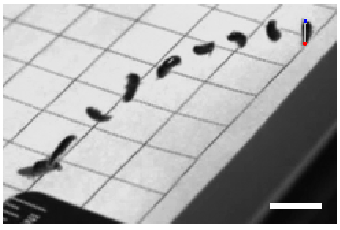
\includegraphics{figures/HyaleTrajectoryPhoto.pdf}
\end{center}
\caption{Representative trajectory, filmed at whatever frame rate.}
\end{figure}

\begin{figure*}
\begin{center}
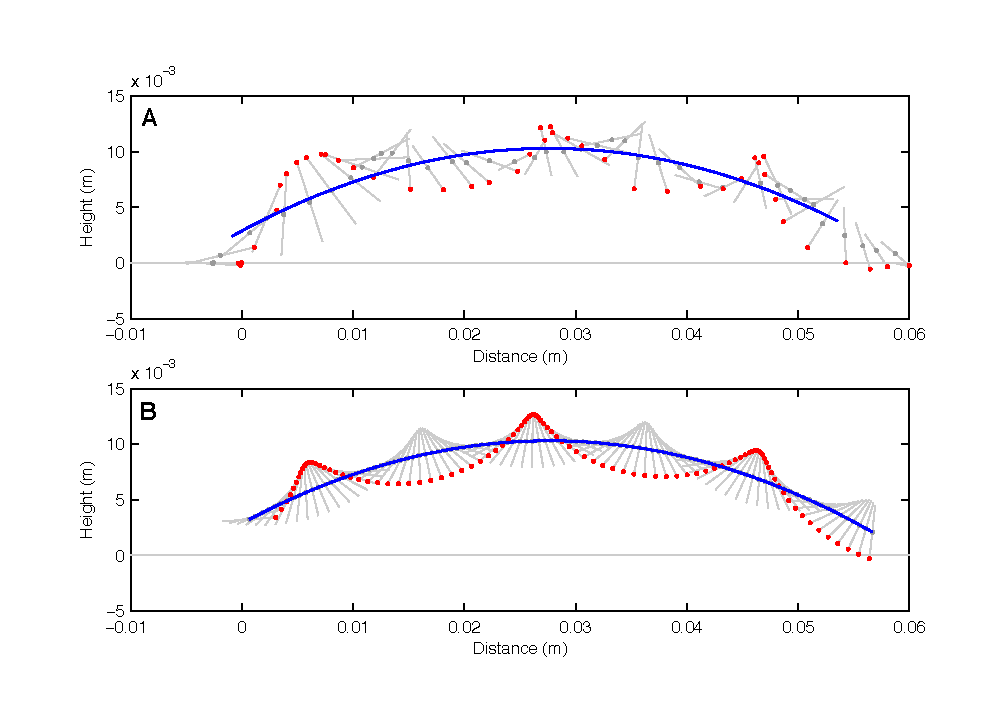
\includegraphics{figures/AmphipodTrajectoriesFull.pdf}
\end{center}
\caption{Comparison of trajectory and model.}
\end{figure*}

%
%\begin{figure}
%\caption{Frames from a typical jump sequence, filmed at \unitfrac[1000]{frames}{s}.  Elapsed time in milliseconds shown at bottom right corner.}
%\label{fig:6}
%\end{figure}

%\begin{figure}
%\caption{\Hyale jump trajectories.  A.  Trajectory from filming at \unitfrac[1000]{frames}{s} in natural light.  Raw video frames shown in Fig.~\ref{fig:6}.  Head shown with blue dots, tail shown with red dots.  Approximate body positions indicated with cartoon from \citep{Kozloff:1996}.  B.  Predicted trajectory using analytical model for initial \unit[3]{ms} of jump with ballistics of spinning rod for remaining trajectory.  Comparison of jump parameters given in Table~\ref{table:x}}
%\label{fig:7}
%\end{figure}

%\begin{figure}
%\caption{Example check of movement of center of mass in $x$ and $y$.  Blue dots indicate measured center of mass positions $x$ and $y$, plotted against time $t$ .  Red line indicates linear regression fit to ballistics in air with gravity, $x = u_0 t + x_0$ and $y = \frac{1}{2} g t^2 + v_0 t + y_0$.  This was repeated for three trajectory.  The minimum $r^2=0.8838$ and maximum $p=3.3\times10^{-16}$.  Jump duration is approximately \unit[60]{ms}.}
%\label{fig:8}
%\end{figure}

\begin{table}
\caption{ Check of fit of trajectory data to simple ballistics using linear regression.  High $r^2$ values mean most of the variance explained by the ballistic model.  In addition, the acceleration term in the $y$-direction matches what would be expected for normal gravitational acceleration.  Parameter estimates are listed as estimate $\pm$ 95\% confidence interval from the regression.  Resulting curves given in Fig.~\ref{fig:8}.}
\label{table:2}
\end{table}

\subsection{Jump distances and initial velocities}
	A histogram of jump distances measured by filming from above at 30 frames/s is shown in Fig. 9.  Comparison by site is given in Fig. 10.  Comparison by body size is given in Fig. 11.  Jump data gathered from trajectories at \unitfrac[30]{frames}{s} and \unitfrac[1000]{frames}{s} is summarized in Table 3.  Table 3 also gives initial velocities and rotation rates and takeoff angles and scaling data from ordinary least squares analysis. 

\begin{figure}
\caption{ Distribution of Hyale jump distances.  A.  Jump distances for Hyale collected from Friday Harbor, 0.061 � 0.025 m (mean � s.d.), for  61 jumps by five individuals in 29 bouts. B.  Jump distances for larger Hyale collected from Cattle Point, 0.038 � 0.019 m for 25 jumps by three individuals in eight bouts.  C.  Polar plot of jump distance and direction, Friday Harbor in blue, Cattle Point in red.  Jumps do not appear to have a preferred direction.}
\label{fig:9}
\end{figure}

\begin{figure}
\caption{Comparison of jump distances for Hyale from Friday Harbor and Cattle Point.  Larger Cattle Point Hyale jump shorter distances (one-way ANOVA, p=5e-5, n=61 Friday Harbor jumps, 25 Cattle Point jumps).  Mean shown with red bar.  Red cross denotes outlier.  Bars indicate lower quartile, median, and upper quartile values. Whiskers extend to 1.5 times the interquartile range.}
\label{fig:10}
\end{figure}

\begin{figure}
\caption{Allometry of Hyale jump distances, Friday Harbor in blue, Cattle Point in red.  Jump distances are shorter in larger individuals.  A.  Jump distance versus body length.  B.  Jump distance versus body mass.  Analysis of covariance revealed no differences between the scaling of individuals from the two sites, so they were collapsed onto the lines shown.   Allometric relationships from ordinary least squares shown on graphs.  Slope is significant ($p=0.0025$).  Regression data in Table~\ref{table:3}A. }
\label{fig:11}
\end{figure}

\begin{table}
\caption{Jump distances, initial velocities, and energetics.}
\label{table:3}
\end{table}

Closeup filming was also used to determine movements at the start of the jump.  A typical closeup sequence is shown in Figs.~\ref{fig:12}-\ref{fig:13}. The body flexion angle and body rotation angle are plotted in Fig.~\ref{fig:14}.  
\begin{figure*}
\begin{center}
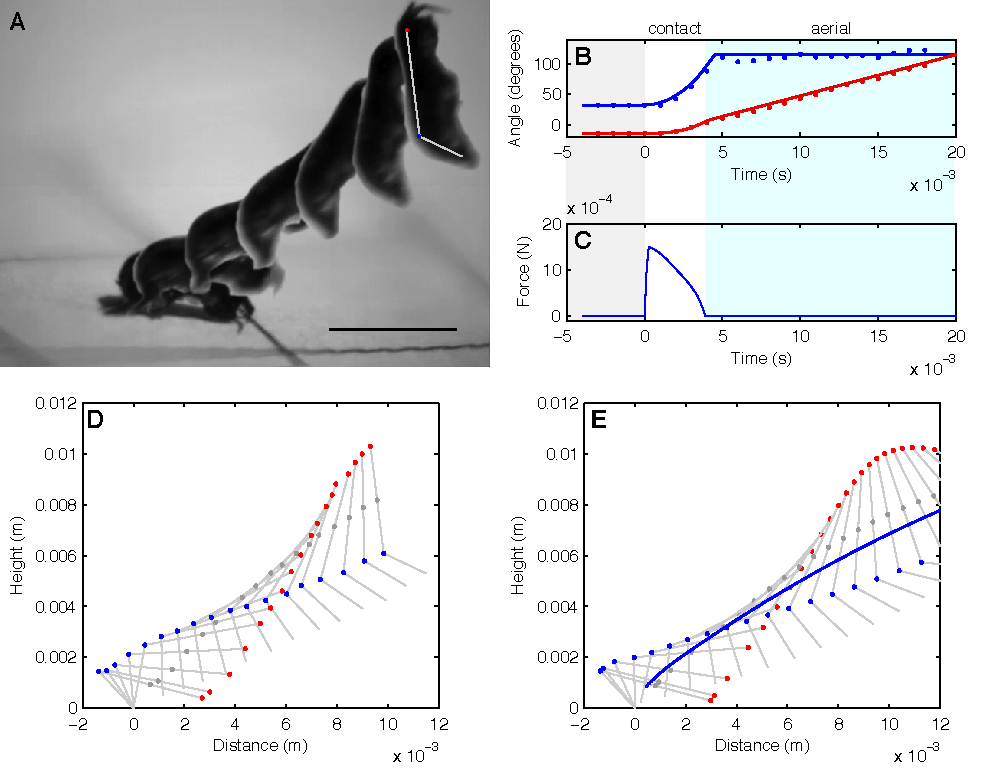
\includegraphics{figures/AmphipodLaunchFull.pdf}
\end{center}
\caption{Comparison of trajectory and model during initial 3 ms of launch.}
\end{figure*}

%\begin{figure}
%\caption{Closeup frames of the initial jump in \Hyale, filmed at \unitfrac[1000]{frame}{s} in natural daylight.  Elapsed time in milliseconds shown at bottom right corner.}
%\label{fig:12}
%\end{figure}

%\begin{figure}
%\caption{A.  Measured eye, rump, and tail positions for sequence shown in Fig.~\ref{fig:12}. Cartoon from \citep{Kozloff:1996}.   B.  Simulated positions using analytical model during initial jump.  Vertical ground reaction force shown in inset, liftoff at \unit[3]{ms} marked by red X.  The two plots show comparable body movements in the initial \unit[3]{ms}.}
%\label{fig:13}
%\end{figure}

%\begin{figure}
%\caption{Measured (A) and simulated (B) joint angle between the pleon and pereon. Angle measurements at 1000/second using convention shown.  Liftoff at 3-4 ms shown with a red x.}
%\label{fig:14}
%\end{figure}

\begin{figure}
\caption{Spot shrimp (\Genus{Pandalus danae}) dissection indicating structures used in abdomen extension that could play a role in \Hyale\ jumping. Red line denotes where flexors and extensors meet.  Dashed black line indicates line of hinges on pleurites.  Elastic elements could include the apodemes, sternite, tergite, and condyles (hinges). Varying lines of action of the flexors and extensors across the hinge joints could be a trigger mechanism.}
\label{fig:15}
\end{figure}

\begin{figure}
\caption{A.  Amphipod anatomy indicating possible methods for powering or triggering jumps, from \citep{Schmitz:1991}.  B.  Example confocal microscope photos of \Parhyale, courtesy M. Perry, Patel Lab, Department of Integrative Biology, UC Berkeley.  Imaging of adults is planned in order to examine the microanatomy used in jumping amphipods.}
\label{fig:16}
\end{figure}

\subsection{Simulations}
	An example simulation is shown in Figs.~\ref{fig:7}B and \ref{fig:13}B.  Parameters for the simulation, obtained from measured and filmed specimens, are given in Table~\ref{table:4}.  The predicted initial velocity and takeoff angle is also given in Table~\ref{table:4}.  
	
\begin{table}
\caption{Simulation parameters and results for analytical model described in appendix 2.}
\label{table:4}
\end{table}

\subsection{Swimming and crawling behavior}
	Crawling and swimming sequences are shown in Figs.~\ref{fig:18}, \ref{fig:19}, and \ref{fig:20}.  These are discussed in detail below. 
	
\begin{figure}
\caption{\Hyale\ crawling on paper.  Alternating tripod gait used by pereopods.  Metachronal rowing used by pleopods.  The tail is also used in tail propping, indicated by the orange arrow.  This indicates the need for a better way to translate movies to printed figures.}
\label{fig:18}
\end{figure}

\begin{figure}
\caption{Swimming behaviors in \Hyale.  A.  Swimming starts with a tail flick in which the pleon is rapidly extended, indicated by the orange arrow.  The tail is also flicked repeatedly during swimming.  The pleopods also beat.  B.  Tail used to pop out of water and loop, indicated by orange arrow.}
\label{fig:19}
\end{figure}

\begin{figure}
\caption{Stick-swim behavior.  \Hyale\ is crawling in a water film on an inverted petri dish.  The laterally compressed body form is used to adhere to the dish, while swimming motion is co-opted to allow forward translation along the surface. }
\label{fig:20}
\end{figure}


\subsection{Anatomy}
Fill this in.  We think its muscles and a snap through mechanism. Detailed anatomical studies of a \unit[5]{mm} animal were not possible during the study period, and the treatment of amphipod abdominal muscles in anatomical texts \citep{Schmitz:1991} was only cursory.  However, dissection of a spot shrimp (\Genus{Pandalus danae}, Fig. 15) suggested several candidates for energy storage mechanisms.  In spot shrimp, the abdominal extensor muscles are small, taking up only a third of the cross section of abdominal muscles.  This is similar to amphipods \citep{Schmitz:1991}.  Based on power output, the abdominal muscles are rejected as the sole power source of jumps.  However, these muscles insert at intersegmental membranes which could provide spring storage.  Alternatively, spring elements could be present in the hinges between abdominal segments, on the pleurites, or a compression spring element could be present in the abdominal sternites.  Another alternative could be pressurization of hemolymph, however, the spot shrimp did not appear to have piping suitable for this means of tail extension. 
	
In addition to a spring, a trigger is needed.  The relationship between muscle axis and bending axis is unclear - in spot shrimp, the flexors and extensors met at an axis that was dorsal to the location of hinges in the pleurites (Fig.~\ref{fig:15}).  This might suggest a trigger mechanism based on changes in the line of action of a force.  Alternatively, a catch mechanism could be used.  In \Hyale, the last pair of periopods were observed to move immediately before jumping, and a latch mechanism on the coxa is feasible.    
	
FIX ME Future work will examine these possibilities using confocal microscopy of a related species, \Parhyale, in cooperation with M. Perry of the Patel Lab at UC Berkeley. 


\section{Discussion}
\subsection{\Hyale\ is a passive spinning rod when in the air}
	  The results suggest that \Hyale\ does not control its trajectory in the air by steering.  This finding agrees with \citet{Bracht:1980}, who saw no means of correcting posture or trajectory in the air.  \Hyale\ retains the ability to swim, and so paddle-like appendages remain small, sized for fluid forces.   However, unlike in bristletails or various wingless insects, \Hyale\ do not perform aerial behavior. 

\subsection{Jump distance and power requirements suggest amphipods have an energy storage mechanism}
The kinetic energy at launch was computed from the initial translational and rotational velocity, body mass, and moment of inertia.  Mass measurements were used to examine the effect of body size.  Larger animals jump shorter distances, however, the data are noisy.  Size scaling and jump scaling data are shown in Figs.~\ref{fig:4} and ref{fig:11}.
	
The cost of transport was also computed, by dividing the initial energy by mass and length of the jump.  For the short jump shown in figure~\ref{fig:7}, the cost of transport was \unitfrac[6]{J}{kg-m}.  The average cost of transport was close to the theoretical minimum (Appendix 1) for jumping, \unitfrac[4.9]{J}{kg-m}.  Compared to other forms of terrestrial locomotion, jumping is expensive per meter of travel because of the wasted energy in raising the center of mass during the flight phase.  However, jumping is fast, at about \unitfrac[100]{body length}{s} for \Hyale.  Jumping also allows movement uphill, and on downhills, jump range is increased. 
	
Is \Hyale\ heroic?  Table~\ref{table:6} provides a comparison with other small jumpers.  In terms of average acceleration and takeoff speed, \Hyale\ is not exceptional compared to other similarly sized jumpers.  \Hyale\ can jump only about half as fast as the more derived \Genus{Orchestia}, and other terrestrial amphipods have up to ten times more range.  

\begin{table}
\caption{Comparison of Hyale with other jumpers.}
\label{table:6}
\end{table}
	
\Hyale\ does have at least one superpower, however.  Like other jumpers, the mass-specific muscle power output required is very high.  \citet{Bennet-Clark:1975} calculated the mass specific power output by dividing the initial kinetic energy by the contact time and the muscle mass (assumed to be 10\% of body mass).  By \citeauthor{Bennet-Clark:1975}'s method \citeyear{Bennet-Clark:1975}, \Hyale\ must produce an average muscle power output of \unitfrac[1078]{W}{kg}, assuming extensor musculature is 10\% of body mass.  This high value is comparable to extreme performers like fleas and trap-jaw ants, and suggests an energy storage mechanism must be at work.  
	
Future work should examine the energy storage mechanism in further detail.  With estimated forces of \unit[1]{mN} occurring over a \unit[3]{ms} period, it will be difficult to directly measure forces exerted by the body.  One possibility is to use photoelastic gelatin \citep{Full:1995}.   However, the analytical model appears to track well with observed kinematics (Fig.~\ref{fig:7} for overall trajectory, Figs.~\ref{fig:13, fig:14} for the instant of launch including contact phase).  With further details of the abdominal musculature, the model torques and joint rotational velocities could be translated into muscle force and shortening velocity, or equivalent stiffnesses of energy storage elements.  The model could be used to evaluate tradeoffs during evolution, specifically changes in morphology between early-branching \Hyale\ and more derived, semi-terrestrial and terrestrial talitrid amphipods.  In addition, the model could be used to examine the relationship between jumping and other modes of locomotion, discussed below.  The model would also be applicable to other jumpers that use abdominal extension, such as springtails and bristletails. 
	
\subsection{Relationship between jumping and other modes of locomotion}
Jumping in amphipods appears to be accomplished with co-opted movements of the tail.  To inform theories about the evolution of jumping in amphipods, amphipods were filmed using their tails for other behaviors tied to locomotion, reported here.  The behaviors observed suggest it is not so clear that jumping is derived solely from escape swimming. 
	
\Hyale\ crawling on paper (a rough substratum) appear to use three different gaits simultaneously (Fig. ~\ref{fig:18}).  In the forward half of the body, the pereopods employ an alternating tripod gait.  The after half (pleosome and urosome) mixes use of a forward-going metachronal rowing wave with the pleopods with tail-propping of the urosome.  In other words, amphipod crawling is like a cockroach, crossed with a millipede and a kangaroo.  It is unclear what the effect of this combination is on the energetics of moving on land.  For typical terrestrial legged locomotion, the mechanical cost of transport is about \unitfrac[1]{J}{kg-m} \citep{Full:2001}, while optimal ballistic jumps should cost \unitfrac[4.9]{J}{kg-m} (derivation in Appendix 2).  However, on the level, \Hyale\ jump even when not pursued.  One possibility to explore in future work is that mixed-gait amphipod crawling is more costly than usual legged gaits, encouraging use of the jump.  Alternatively, \citep{Schmitz:1991} proposed that the condyles in amphipod legs are poorly developed, limiting leg performance.
	
In water, tail extension is used to start swimming and tail flicks occur periodically during swimming (Fig. 19A).  Pleopod rowing is also used during swimming.  The relationship between swimming and jumping could be explored with the simulation model, by adding fluid loads onto the links and comparing observed and simulated kinematics.  This is currently underway. 
	
The most interesting uses of the tail occurred near solid bottoms and free surfaces.  \Hyale\ were observed to use the tail for looping turns and to pop out of water (Fig.~\ref{fig:19}B).  The tail was also used during sideways swimming and during a related mode of �stick-swimming� in which a sideways animal adhered to a surface and used swimming motions of the tail to propel itself (Fig.~\ref{fig:20}).  Stick-swimming was observed on glass and plexiglass on the level, at 90\degree\ inclines, and inverted.   \Hyale\ used stick-swimming in thin films on rocks and when stuck to kelp.  In several instances, animals appeared to easily right themselves and then re-stick on the opposite side of the body.  \Hyale\ used stick-swimming to escape from a grasping human by shuffling along walls and at the bottom corner of petri dishes.  Examination of the biomechanics of stick-swimming using modeling is currently underway.  
	
Future work should also look at surface properties of the cuticle.  Amphipods must retain a film and allow adhesion and yet avoid water loss.  Also, amphipods jumping on very smooth surfaces seemed not to launch as effectively due to slippage.   
	
The results of this project have suggested future work to tie together the mechanics of jumping, the anatomy, other modes of locomotion, and ecological context for terrestrial behavior in amphipods.  Talitrid amphipods are a good system in which to perform such studies in because they are compact, their ecology is contained within the intertidal zone, phylogenies are improving, these amphipods are a lineage that recently invaded land, with members that are fully marine, freshwater, and terrestrial, and they occur in exotic destinations worldwide, including giant forms in the deep sea and Antarctic.    

\section{List of symbols}
\begin{jebsymbolslist}
\item[x] Something here.
\end{jebsymbolslist}

\section{Appendix 1: Math model of the initial launch}
\label{app:1}
	The jumping amphipod body is modeled as two rigid planar links.  The links have rotational inertias $J_1$ and $J_2$ for the distal and proximal links, masses $m_1$ and $m_2$, lengths $l_1$ and $l_2$, and centers $r_1$ and $r_2$ (assumed to be $l_1/2$ and $l_2/2$, respectively).  The pin joint at the ground is free to rotate, while the pin joint between the links is acted on by a torque due to the musculoskeletal system, modeled as a spring and a damper.  The state of the link is completely specified by the joint angles $\theta_1$ and $\theta_2$.  To simplify the algebra, the joint angles are specified as relative joint angles between links.  

	The equations of motion are derived from Lagrange's equations, in which a function relating kinetic and potential energy is differentiated to obtain system dynamics \citep{Baruh:2007}.  $T^*$ is the kinetic energy, $V$ is potential energy, $q$ are generalized state variables, and $t$ is time. 
\begin{equation}
\mathcal{L} = T^* - V
\end{equation}
\begin{equation}
\frac{d}{dt}\frac{\partial \mathcal{L}}{\partial \dot{q}}
-
\frac{\partial \mathcal{L}}{\partial q}
=
Q
\end{equation}

	For small bodies, the potenial energy $V$ due to changes in height will be small, and it is ignored in this model.  $T^*$, the kinetic energy of the links is given by the lengths, masses, inertias, and instantaneous state:
\begin{equation}
T^* = \frac{1}{2}m_1 v_1^2 +
\frac{1}{2}J_1 \omega_1^2 +
\frac{1}{2}m_2 v_2^2 +
\frac{1}{2}J_2 \omega_2^2
\end{equation}
where the velocities are all functions of the joint angles, joint angular velocities, and lengths of the linkages.  The full derivation is available in  \citep{Baruh:2007};  here I provide a sketch of the result.  Applying Lagrange's equations results in the following second order differential equation:
\begin{equation}
M_A 
\left[ \begin{array}{c}
\ddot\theta_1 \\
\ddot\theta_2
\end{array} \right]
+ M_B 
\left[ \begin{array}{c}
\dot\theta_1 \\
\dot\theta_2
\end{array} \right]
=
\left[ \begin{array}{c}
\tau_1 \\
\tau_2
\end{array} \right]
\end{equation}
where the components of $M_A$ and $M_B$ are given by
\begin{equation}
M_{A,11} = J_1 + J_2 + m_1 r_1^2 + m_1 (l_1^2 + r_2^2) + m_2 l_1 l_2 \cos\theta_2
\end{equation}
\begin{equation}
M_{A,12} =J_2 + m_2 r_2^2 + \frac{1}{2}m_2 l_1 l_2 \cos\theta_2
\end{equation}
\begin{equation}
M_{A,21} =J_2 + m_2 r_2^2 + \frac{1}{2} m_2 l_1 l_2 \cos\theta_2
\end{equation}
\begin{equation}
M_{A,22} =J_2 + m_2 r_2^2
\end{equation}
and
\begin{equation}
M_{B} =
\left[\begin{array}{cc}
-\frac{1}{2} m_2 l_1 l_2 \sin\theta_2 \dot\theta_2 & 
-\frac{1}{2} m_2 l_1 l_2\sin\theta_2 (\dot\theta_1 + \dot\theta_2) \\
\frac{1}{2}m_2 l_1 l_2 \sin\theta_2\dot\theta_1 &
0
\end{array}\right]
\end{equation}
The joint torques are given by a free pivot at the ground and a damped spring representing the musculoskeletal system at the pereon to pleon joint:
\begin{equation}
\tau_1 = 0
\end{equation}
\begin{equation}
\tau_2 = K_{eff} \theta_2 + B_{eff} \dot{\theta}_2
\end{equation}
This is a second order, nonlinear system of differential equations with variable coefficients.  The second order system can be recast into first order state space canonical form, with state variables $[\theta_1, \theta_2, \dot\theta_1, \dot\theta_2]^T$.  In this form it can be solved by standard solvers for ordinary differential equations, such as Matlab's {\tt ode45}.   

\section{Appendix 2: Mechanical cost of optimal jumping}
For the case of jumping without drag, jumps are modeled by simple ballistics.  The longest jump occurs at 45\degree~according to Tartaglia's Law.  For this trajectory, the initial kinetic energy required is given by:
\begin{equation}
E_0 = \frac{1}{2} m v^2
\end{equation}
where $m$ is mass, and $v$ is velocity.  The range is given by:
\begin{equation}
d = \frac{v^2}{g}
\end{equation}
where  $g = 9.81$ m/s$^2$ is the acceleration of gravity.  Thus, the mechanical cost of jumping, or the energy to move 1 kg of animal 1 m, is given by:

\begin{equation}
COT_{mech} = \frac{E_0}{dm} = \frac{g}{2}
\end{equation}

For an optimal jump starting from rest, the mechanical cost ignoring any rotation is \unitfrac[4.9]{J}{kg-m}.  Energy lost in body rotation will increase the cost.  This cost is 4.9 times the cost reported for walking and running on the level in various fully terrestrial vertebrates and arthropods, \unitfrac[1]{J}{kg-m} \citep{Full:2001}. 

\jebacknowledgements{We thank Emily Carrington, Mark Denny, John Gosline, Katie Mach, and the rest of the Friday Harbor Labs summer biomechanics course 2008 for stimulating discussions, project advice, and the chance to work on amphipods at Friday Harbor.  We also thank Tom Daniel for a high speed camera and lenses; Craig Staude for advice on amphipods and a zoom lens; Nipam Patel, Mimi Koehl and Robert Dudley for useful advice; Wan Lan Chang, Tyler Mason and Chris Neufeld for assistance collecting; and Eric Lambert for help with the filming setup.  DE was funded by a UC Chancellor's Fellowship, UW FHL financial aid, Eric and Mary Horvitz, and the SICB Libby Hyman Award.}

\bibliography{references/amphipod}
\end{document}
